\documentclass{beamer}

\mode<presentation>
{
  \usetheme{CambridgeUS}      % or try Darmstadt, Madrid, ...
  \usecolortheme{default} % or try albatross, beaver, crane, ...
  \usefonttheme{default}  % or try serif, structurebold, ...
  \setbeamertemplate{navigation symbols}{}
  \setbeamertemplate{caption}[numbered]
} 

\usepackage[english]{babel}
\usepackage[utf8x]{inputenc}
\usepackage{listings}
\usepackage[ampersand]{easylist}



\definecolor{KTI_green}{RGB}{150, 189, 13}
\definecolor{TU_red}{RGB}{255, 55, 81}
\definecolor{faint_gray}{RGB}{180, 180, 180}

\definecolor{syntax_green}{rgb}{0,0.6,0}
\definecolor{syntax_gray}{rgb}{0.9, 0.9, 0.9}
\definecolor{syntax_mauve}{rgb}{0.58,0,0.82}

\lstset{ 
  backgroundcolor=\color{syntax_gray},  % choose the background color
  basicstyle=\scriptsize\ttfamily,        		% size of fonts used for the code
  breaklines=false,                		% automatic line breaking only at whitespace
  captionpos=b,                    		% sets the caption-position to bottom
  commentstyle=\color{syntax_green},    % comment style
  escapeinside={\%*}{*)},          		% if you want to add LaTeX within your code
  keywordstyle=\color{blue},       		% keyword style
  stringstyle=\color{syntax_mauve},     % string literal style
  columns=fullflexible,
  frame=single,
  framesep=0.5cm,
  framexleftmargin=0.5cm,
  xleftmargin=0.5cm,
  framexrightmargin=0.5cm,
  xrightmargin=0.5cm,
  frame=tb,                 
    numbers=left,                    
    numbersep=15pt,  
  }
  
  
\newcommand{\logopython}{\raggedleft 
\includegraphics[height=0.5cm]{logo_python}\hspace{0.1cm}\\\raggedright}
\newcommand{\logopythonbottom}{\raggedleft\vspace{-0.8cm}
\includegraphics[height=0.5cm]{logo_python}\hspace*{0.05cm}\\\raggedright}

\title[BSP29 - Bankomat]{Bankomat}
\author{Dickbauer Y., Moser P., Perner M.}
\institute{PS Computergestützte Modellierung, WS 2016/17}
%\date{Date of Presentation}

\begin{document}

\begin{frame}
  \titlepage
\end{frame}

\begin{frame}{Outline}
  \tableofcontents
\end{frame}

\section{Aufgabenstellung}
\begin{frame}{Aufgabenstellung}
Eine Bank muss entscheiden, wie viele Bankomaten installiert werden sollen, wenn alle 60 Sekunden (exponentialverteilt) ein neuer Kunde die Bank betritt. Die Zeit, die ein Kunde am Bankomat verbringt, ist exponentialverteilt mit dem Erwartungswert von 2 Minuten.
\\~\\
Eine Marktuntersuchung ergab, dass sich Kunden dann nicht mehr anstellen, wenn bereits drei oder mehr Personen warten. Die Aufgabenstellung eines Bankomaten beträgt 10.000 Euro; pro Kunde, der den Bankomaten anstelle des Schalters benutzt, spart sich die Bank 10 Cent. Der Bankomat ist täglich 15 Stunden in Betrieb.
\end{frame}

\begin{frame}{Aufgabenstellung}
Simulieren Sie Strategien mit 1,2, und 3 Bankomaten und bestimmen Sie, wie viele Bankomaten aufgestellt werden sollen, damit die Kosteneinsparungen während des ersten Jahres möglichst groß sind.
\\~\\
Hinweis: simulieren Sie einen Tag und rechnen Sie das Ergebnis auf ein Jahr hoch.
\vspace{1cm}
\begin{itemize}
  \item Eingabe: Anzahl an Bankomaten
  \item Output: Warteschlangenlänge am Periodenanfang, Neuankunft (?), Abfertigung in Periode (?), Anzahl an weggegangenen Kunden, Kosten/Nutzenvergleich
\end{itemize}
\end{frame}

\subsection{Verwendete Funktionen}
%\begin{frame}[fragile]{Funktion loaded\_random\_choice(..)}
  \begin{itemize}
    \item Diese Funktion verlangt eine WSKL Liste als Eingabeparameter
    \item Gibt einen Index zurück, welcher 0 bis $\left\vert{probality\_list}\right\vert-1$ sein kann.
    \item Diese Indizes haben eine gewichtete WSKL, welche jeweils an der Position in der Eingabeliste steht
    \item Beispiel probility\_list := [ 0.9, 0.1 ]  $\Rightarrow$ mit p=90\% wird 0 zurückgegeben, p=10\% für 1
  \end{itemize}
  \begin{lstlisting}[language=python]
def loaded_random_choice(probability_list):
    n = len(probability_list)
    random_number = random.random()
    cum_p = 0
    for i in range(n):
        cum_p += probability_list[i]
        if cum_p > random_number:
            return i
    return None
\end{lstlisting}
\logopythonbottom
\end{frame}	

\section{Ergebnisse}
\begin{frame}[fragile]{Simulationsergebnis}
    	\begin{figure}[h!]
    	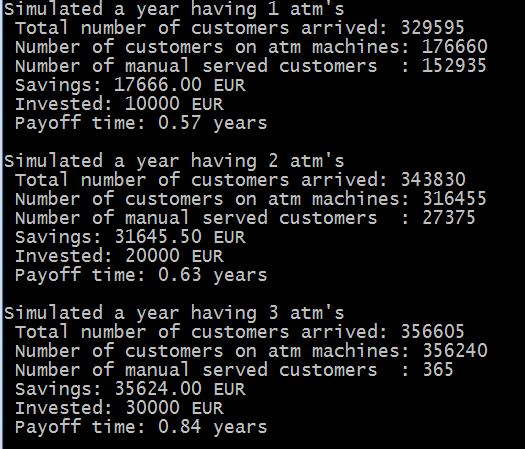
\includegraphics[scale=0.6]{BSP29_Output.PNG}
		\end{figure}
\end{frame}

\end{document}
